\chapter{提案手法}

本章では提案する手法の詳細について説明する.

\section{提案手法の概要}

\begin{figure}[htbp]
\begin{center}
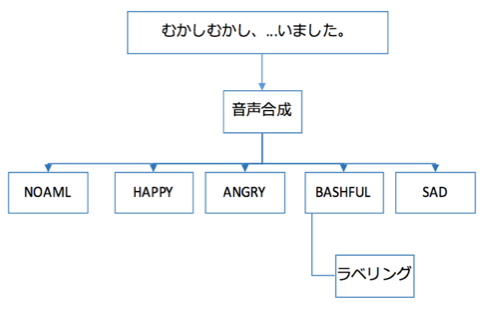
\includegraphics[width=15cm,clip,bb=0 0 349 232]{fig/create_data.png}
\caption{正解データの作成}\label{create_data}
\end{center}
\end{figure}

本手法では予め人手で各文に対して感情ラベルを与えた教師データを作成しそのデータを機械学習することで分類機を作成する.感情ラベルは,普通,嬉しい,恥ずかしい,怒ってる,悲しいの5種類とする.未知の入力文が与えられた場合に,この中の一つを自動的に割り当てることが目的である.
基本的に句点ごとに文章を分割してすべての文がそれぞれのどの感情として音声合成されるべきかを推定する.なお,分割する際は基本的に句読点で分割し,カギカッコの始まりは句読点とみなしてそこから次の文の始まりとした.また,カギカッコ内の句読点も分割の対象とした.ここで文章に依存する内容語による推定では膨大な教師データが必要になると考えられる.そこで内容語によらず文の形式である程度,感情を推定することができると仮定して,文の機能語のみを抽出して学習を行う.具体的には名詞,動詞,形容動詞,形容詞を取り除く.
その後,各文は品詞分解し基本形変換を行いbags of wordsに変換し正解ラベルを元に学習を行う.分類機にはナイーブベイズ,ランダムフォレスト等を用いる予定である.

